\documentclass[conference]{IEEEtran}
\IEEEoverridecommandlockouts

\usepackage{cite}
\usepackage{amsmath,amssymb,amsfonts}
\usepackage{graphicx}
\usepackage{textcomp}
\usepackage{xcolor}
\usepackage{booktabs}
\usepackage{array}
\usepackage{tikz}
\usetikzlibrary{shapes.geometric, arrows.meta, positioning}

\def\BibTeX{{\rm B\kern-.05em{\sc i\kern-.025em b}\kern-.08em
    T\kern-.1667em\lower.7ex\hbox{E}\kern-.125emX}}

\begin{document}

\title{RF-Based Drone Identification Using Machine Learning: Presence,
Family and Operating-Condition Classification}

\author{
\IEEEauthorblockN{Utkarsh Sinha}
\IEEEauthorblockA{Dept. of Electronics and\\Telecommunication\\
BMS College of Engineering\\Bengaluru, India\\1BM23ET055}
\and
\IEEEauthorblockN{Vishal Joshy}
\IEEEauthorblockA{Dept. of Electronics and\\Telecommunication\\
BMS College of Engineering\\Bengaluru, India\\1BM23ET058}
\and
\IEEEauthorblockN{Yash Gupta}
\IEEEauthorblockA{Dept. of Electronics and\\Telecommunication\\
BMS College of Engineering\\Bengaluru, India\\1BM23ET061}
\and
\IEEEauthorblockN{Dr. C Gururaj}
\IEEEauthorblockA{Professor\\Ph.D., M.Tech\\
Dept. of Electronics and\\Communication\\
BMS College of Engineering\\gururaj.tce@bmsce.ac.in}
}

\maketitle

\begin{abstract}
Detecting and identifying drones from the radio-frequency (RF) signals they
exchange with their controllers is a passive alternative to vision- or
radar-based surveillance that works without line of sight or favourable
lighting. This project builds a machine-learning pipeline that uses the public
\textbf{DroneRF} dataset to answer three questions from a recorded RF segment:
is a drone present, which drone family is it, and which recorded operating
condition is most likely. Raw captures from the 2.4~GHz ISM band are segmented
and converted into a 2048-point power-spectrum feature vector using the Fast
Fourier Transform across the low and high RF sub-bands. Four classical
classifiers --- Logistic Regression, Random Forest, Support Vector Machine with
an RBF kernel, and XGBoost --- are compared on each task under a leakage-aware
evaluation that groups all segments of one recording into the same fold. On a
held-out evaluation, drone \emph{presence} is detected with a macro-F1 of up to
1.000, drone \emph{family} (background, Parrot Bebop, Parrot AR, DJI Phantom)
reaches a macro-F1 of 1.000 for XGBoost, and the harder 10-class
\emph{operating-condition} task reaches a macro-F1 of 0.492 for XGBoost under
5-fold cross-validation, clearly above the $\sim$0.37 linear and bagging
baselines. A noise-robustness test shows family accuracy degrades from 0.900 on
clean data to 0.294 at $-5$~dB SNR, quantifying sensitivity to the Wi-Fi and
Bluetooth interference that shares the band. The system is intended as an
interpretable, low-cost, dataset-based decision-support tool and not as a
deployed counter-drone system.
\end{abstract}

\begin{IEEEkeywords}
Drone detection, RF fingerprinting, UAV identification, machine learning,
DroneRF, XGBoost, feature extraction, power spectral density, data leakage.
\end{IEEEkeywords}

\section{Introduction}
Unmanned aerial vehicles (UAVs), or drones, are now inexpensive and widely
available, and their misuse raises privacy, safety and security concerns around
airports, public events and restricted areas. Reliable detection and
identification of an intruding drone is therefore an important problem.

Visual and acoustic sensing require line of sight and favourable conditions,
and active radar can be costly. Drones, however, continuously communicate with
their flight controllers over wireless RF links, usually in the 2.4~GHz
industrial, scientific and medical (ISM) band. Passively listening to these RF
signals allows detection without cooperation from the drone and without line of
sight.

Knowing only that \emph{some} drone is present is of limited value. A useful
system should also indicate \emph{which} drone and, ideally, \emph{what} it is
doing, since different models and flight modes imply different threats. This
project therefore develops a machine-learning pipeline that uses recorded
DroneRF signals to perform three progressively harder classification tasks ---
presence, family and operating condition --- and compares four classical
machine-learning algorithms on each.

\section{Overview}
The system analyses recorded RF segments and produces three predictions. The
three classification targets are defined as:
\[
\text{presence} \in \{0,1\},\quad
\text{family} \in \{0,1,2,3\},\quad
\text{mode} \in \{0,\dots,9\}.
\]
where \emph{presence} is drone vs.\ no-drone, \emph{family} distinguishes
background and three drone types, and \emph{mode} identifies the specific
recorded operating condition.

The basic operation of the system can be summarized as:

\noindent\textbf{Raw RF Captures $\rightarrow$ Segmentation $\rightarrow$
FFT Feature Extraction $\rightarrow$ Label Decoding $\rightarrow$ Model Training
(4 classifiers) $\rightarrow$ Leakage-Aware Evaluation}

The data comes from a single public source:
\begin{itemize}
\item The DroneRF dataset \cite{dronerf_dib, alsad_fgcs}.
\end{itemize}

Each capture is labelled by a 5-digit \emph{BUI} code embedded in its filename.
All three targets are decoded from this single code, so no manual labelling is
required. Because each target has a small number of discrete classes, every
task is a classification problem, not a regression problem.

\section{Problem Statement}
The presence of a drone cannot be reliably read from a single sensor in all
conditions, yet knowledge of it is essential for security and airspace
management. RF sensing is passive and works without line of sight, but
real-world signals in the 2.4~GHz band are shared with Wi-Fi and Bluetooth,
which makes the classification task noisy.

In addition, RF classifiers trained and tested carelessly can report
optimistic results because many segments extracted from one physical recording
are highly correlated; if such segments are split across training and test
sets, the model effectively sees the test data during training. Therefore,
there is a need for a data-driven system that classifies drone presence, family
and operating condition from easily computed spectral features, and whose
evaluation explicitly avoids this data leakage.

The proposed system uses classical machine learning to classify RF segments
from the DroneRF dataset, and evaluates the trained models under a
recording-grouped split and under added noise.

\section{Literature Survey}
Many studies have investigated RF-based drone detection and identification using
machine learning. Early work established the dataset and deep-learning baseline;
later work explored feature engineering, interference robustness and
lightweight deployment.

\subsection{Dataset and Deep-Learning Baseline}
Al-Sa'd et al.\ \cite{alsad_fgcs} introduced the DroneRF dataset and trained
deep neural networks for detection, type and mode classification, establishing
the three-task structure used here. The accompanying data descriptor
\cite{dronerf_dib} documents the file structure and BUI labelling scheme.

\subsection{Classical Machine Learning Approaches}
Al-Emadi et al.\ \cite{alemadi_xgb} applied XGBoost to the same three tasks and
reported average accuracies of 99.96\%, 90.73\% and 70.09\% for detection, type
and mode respectively, confirming that tree-boosting is strong on this data.
Ezuma et al.\ \cite{ezuma_micro} classified UAV controllers from RF fingerprints
using statistical features and classifiers such as k-nearest neighbours.

\subsection{Interference and Robustness}
Ezuma et al.\ \cite{ezuma_interf} studied detection and classification in the
presence of Wi-Fi and Bluetooth interference. Recent journal work continues
this theme: robustness of RF UAV detectors \cite{robust_sensors}, ensemble
fingerprinting under jamming \cite{ensemble_sensors}, and low-SNR recognition
with complex-valued networks \cite{cvcnn_sensors}.

\subsection{Feature Extraction Alternatives}
Medaiyese et al.\ \cite{medaiyese_wavelet} used wavelet-transform features, and
the LUMEN framework \cite{lumen_sensors} used power-spectral-density features
similar to those used here. These works motivate the spectral feature choice of
this project.

\subsection{Comparative Analysis}
Table~\ref{tab:litcompare} summarizes representative works against the proposed
system.

\begin{table}[t]
\centering
\caption{Literature Comparison}
\label{tab:litcompare}
\footnotesize
\begin{tabular}{@{}p{1.6cm}p{2.0cm}c p{1.8cm}@{}}
\toprule
\textbf{Reference} & \textbf{Method} & \textbf{Year} & \textbf{Focus} \\
\midrule
Al-Sa'd et al.\ \cite{alsad_fgcs} & Deep neural network & 2019 & DroneRF dataset + 3 tasks \\
Al-Emadi et al.\ \cite{alemadi_xgb} & XGBoost & 2020 & Detect / type / mode \\
Ezuma et al.\ \cite{ezuma_interf} & ML + interference & 2020 & Robustness to Wi-Fi/BT \\
Medaiyese et al.\ \cite{medaiyese_wavelet} & Wavelet + ML & 2022 & Feature extraction \\
LUMEN \cite{lumen_sensors} & PSD + lightweight net & 2026 & Edge deployment \\
\textbf{Proposed} & \textbf{4 classical ML, FFT features} & \textbf{2026} & \textbf{Leakage-aware 3-task comparison} \\
\bottomrule
\end{tabular}
\end{table}

\subsection{Research Gap}
Much existing work either focuses on deep learning or reports high accuracy
without explicitly controlling for segment-level data leakage. This project
addresses the gap by comparing four interpretable classical models across all
three tasks under a recording-grouped split, and by quantifying noise
robustness directly.

\section{Libraries and Tools Used}
\textbf{Python 3.11.} Python is the core language used for preprocessing,
feature extraction, model training, evaluation and plotting.

\begin{itemize}
\item \textbf{NumPy} --- FFT, array operations and the power-spectrum feature
computation.
\item \textbf{Pandas} --- loading and organizing the feature table, and writing
it to a columnar Parquet file.
\item \textbf{scikit-learn} --- Logistic Regression, Random Forest, SVM,
the grouped train/test split (\texttt{GroupKFold} / \texttt{GroupShuffleSplit})
and the metrics (precision, recall, F1, confusion matrix).
\item \textbf{XGBoost} --- the gradient-boosted tree classifier.
\item \textbf{Matplotlib} --- confusion-matrix heatmaps and the
noise-degradation curve.
\item \textbf{Kaggle API} --- reproducible download of the DroneRF dataset.
\end{itemize}

\section{System Design and Methodology}
Fig.~\ref{fig:block} shows the proposed pipeline.

\begin{figure}[t]
\centering
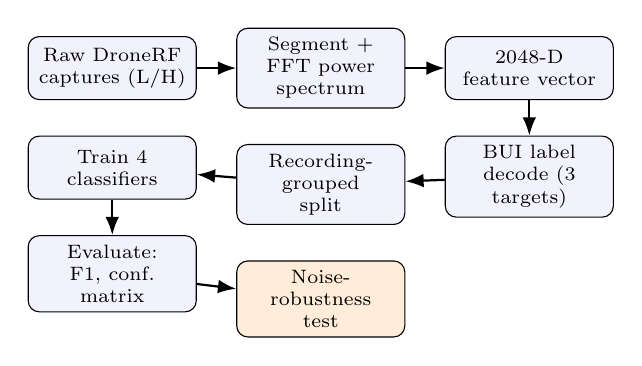
\begin{tikzpicture}[
  node distance=0.45cm and 0.5cm,
  box/.style={rectangle, draw, rounded corners, align=center,
    font=\scriptsize, minimum height=0.8cm, text width=1.9cm, fill=blue!5},
  save/.style={rectangle, draw, rounded corners, align=center,
    font=\scriptsize, minimum height=0.8cm, text width=1.9cm, fill=orange!15},
  arr/.style={-{Latex}, thick}
]
\node[box] (raw) {Raw DroneRF\\captures (L/H)};
\node[box, right=of raw] (seg) {Segment +\\FFT power spectrum};
\node[box, right=of seg] (feat) {2048-D\\feature vector};
\node[box, below=of feat] (label) {BUI label\\decode (3 targets)};
\node[box, below=of seg] (split) {Recording-grouped\\split};
\node[box, below=of raw] (train) {Train 4\\classifiers};
\node[box, below=of train] (eval) {Evaluate:\\F1, conf.\ matrix};
\node[save, below=of split] (noise) {Noise-robustness\\test};
\draw[arr] (raw) -- (seg);
\draw[arr] (seg) -- (feat);
\draw[arr] (feat) -- (label);
\draw[arr] (label) -- (split);
\draw[arr] (split) -- (train);
\draw[arr] (train) -- (eval);
\draw[arr] (eval) -- (noise);
\end{tikzpicture}
\caption{System flow diagram.}
\label{fig:block}
\end{figure}

\subsection{Raw Data}
The DroneRF dataset contains recorded RF activity for background (no drone) and
three drones: Parrot Bebop, Parrot AR and DJI Phantom. Each capture is stored as
two CSV files, a low sub-band (\texttt{L}) and a high sub-band (\texttt{H}), of
the 2.4~GHz band. There are 227 recording pairs in total.

\subsection{Label Decoding}
Each file name begins with a 5-digit BUI code. The code encodes all three
targets simultaneously, as summarized in Table~\ref{tab:bui}. Presence is 0 for
background and 1 otherwise; family maps the code to one of four classes; mode is
a distinct index for each of the ten BUI codes.

\begin{table}[t]
\centering
\caption{BUI Code to Labels}
\label{tab:bui}
\footnotesize
\begin{tabular}{@{}llp{3.2cm}@{}}
\toprule
\textbf{BUI code(s)} & \textbf{Family} & \textbf{Meaning} \\
\midrule
00000 & 0 & Background, no drone \\
10000--10011 & 1 & Bebop (4 modes) \\
10100--10111 & 2 & AR drone (4 modes) \\
11000 & 3 & Phantom (1 mode) \\
\bottomrule
\end{tabular}
\end{table}

\subsection{Feature Extraction}
Each capture is divided into non-overlapping segments of $L = 100{,}000$
samples. For a segment $x$, the mean is removed and a 2048-point FFT magnitude
is computed, keeping the upper half ($M/2 = 1024$ bins):
\[
X_f = \big|\,\mathrm{FFT}_{M}(x - \bar{x})\,\big|,\qquad
f = \tfrac{M}{2}+1,\dots,M.
\]
The low- and high-band spectra are concatenated with a continuity scaling and
squared to give a power spectrum, producing a 2048-dimensional feature vector
per segment. The complete dataset yields 22{,}700 feature vectors.

\subsection{Leakage-Aware Split}
Because all segments of one capture are highly correlated, the evaluation groups
every segment of a recording into the same fold using \texttt{GroupKFold}
(5 folds) or a single 75/25 grouped split. This prevents segments from one
recording appearing in both training and test sets.

\subsection{Classifiers}
Four models are trained and compared on each task: Logistic Regression (a linear
baseline), Random Forest (a bagging ensemble of trees), SVM with an RBF kernel
(for curved class boundaries, trained on a 5000-sample subset for tractability),
and XGBoost (gradient-boosted trees).

\subsection{Evaluation Metrics}
For each model and task we report macro-averaged precision, recall and F1, and a
confusion matrix. Macro-F1 is used as the headline metric because the classes
are imbalanced:
\[
\text{F1} = \frac{2\,PR}{P+R},\qquad
\text{macro-F1} = \frac{1}{K}\sum_{k=1}^{K}\text{F1}_k .
\]

\section{Results and Discussion}
Table~\ref{tab:results} reports macro-F1 for every model and task. Presence and
family are reported on a single grouped split; the harder mode task is reported
as mean $\pm$ standard deviation over 5 folds.

\begin{table}[t]
\centering
\caption{Macro-F1 by Model and Task}
\label{tab:results}
\footnotesize
\begin{tabular}{@{}lcccc@{}}
\toprule
\textbf{Task} & \textbf{LR} & \textbf{RF} & \textbf{SVM} & \textbf{XGBoost} \\
\midrule
Presence & 1.000 & 0.978 & 1.000 & 1.000 \\
Family & 0.999 & 0.898 & 0.977 & \textbf{1.000} \\
Mode (5-fold) & 0.375 & 0.378 & 0.160\textsuperscript{*} & \textbf{0.492} \\
\bottomrule
\end{tabular}
\\[2pt]
\footnotesize\textsuperscript{*}SVM trained on a 5000-sample subset per fold.
\end{table}

Presence detection is essentially solved by all models. Family classification is
also solved by XGBoost, whose confusion matrix (Fig.~\ref{fig:cm}) is a perfect
diagonal. The 10-class mode task is substantially harder; XGBoost reaches a
macro-F1 of 0.492, clearly above the linear and bagging baselines around 0.37,
making it the best model on the task that matters most.

\begin{figure}[t]
\centering
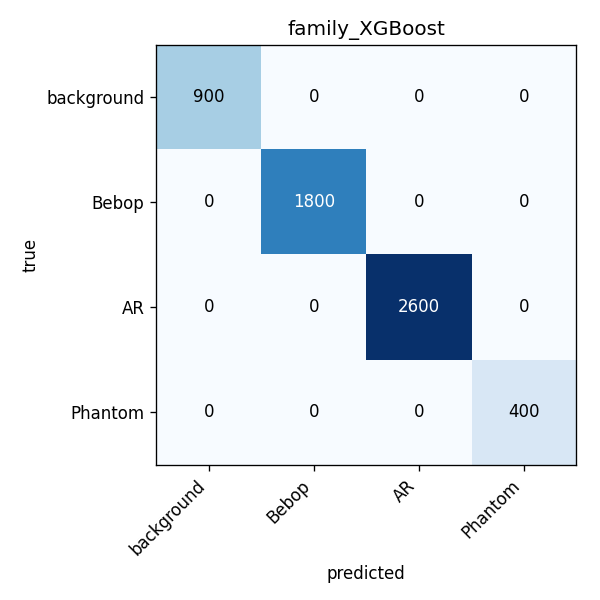
\includegraphics[width=0.46\columnwidth]{figs/cm_family.png}\hfill
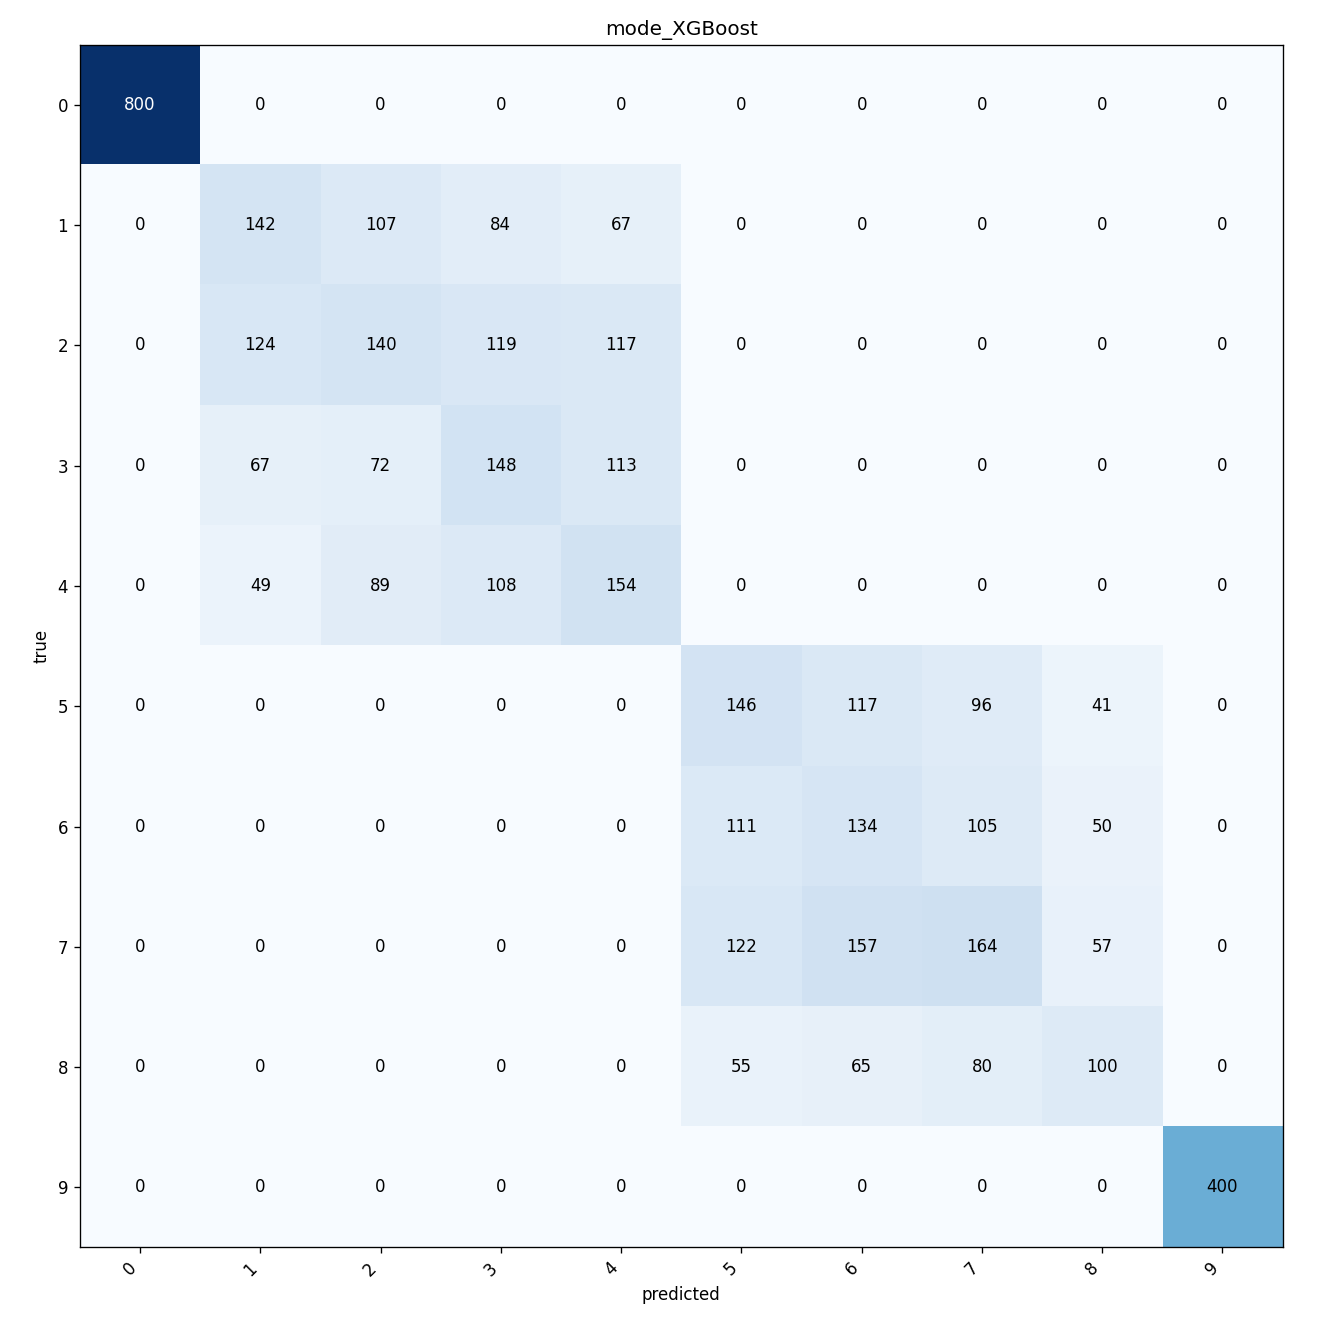
\includegraphics[width=0.46\columnwidth]{figs/cm_mode.png}
\caption{XGBoost confusion matrices: family (left, perfect) and mode (right,
10-class).}
\label{fig:cm}
\end{figure}

\subsection{Noise Robustness}
To test the interference concern of the 2.4~GHz band, Gaussian noise was added
to the test features at decreasing SNR for the family task
(Table~\ref{tab:noise}, Fig.~\ref{fig:noise}). Accuracy falls from 0.900 on
clean data to about 0.50 at 20~dB and 0.29 at $-5$~dB, showing that spectral
features alone are not robust to heavy noise and that explicit interference
handling would be needed for deployment.

\begin{table}[t]
\centering
\caption{Family Macro-F1 vs.\ SNR (Random Forest)}
\label{tab:noise}
\footnotesize
\begin{tabular}{@{}lcccccc@{}}
\toprule
SNR & clean & 20 dB & 10 dB & 5 dB & 0 dB & $-5$ dB \\
\midrule
Macro-F1 & 0.900 & 0.496 & 0.424 & 0.376 & 0.320 & 0.294 \\
\bottomrule
\end{tabular}
\end{table}

\begin{figure}[t]
\centering
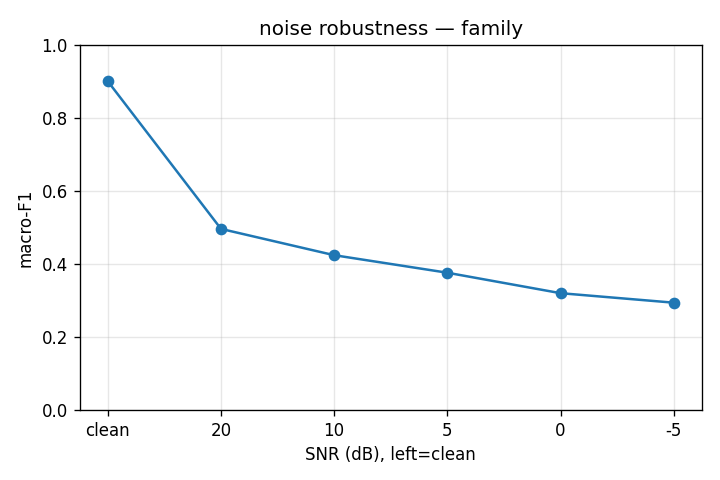
\includegraphics[width=0.75\columnwidth]{figs/noise.png}
\caption{Noise-robustness curve for the family task.}
\label{fig:noise}
\end{figure}

\subsection{Fair-Evaluation Note}
The near-perfect presence and family scores are honest given the
recording-grouped split, but residual correlation between captures of the same
mode may remain. The small 5-fold standard deviation ($\pm0.009$) indicates the
results are stable rather than the product of a single lucky split.

\section{Conclusion}
This project built and evaluated a classical machine-learning pipeline for
RF-based drone identification on the DroneRF dataset. Four models were compared
across presence, family and operating-condition classification under a
leakage-aware split. Presence and family are reliably classified, while the
10-class operating-condition task remains hard, with XGBoost giving the best
macro-F1 of 0.492. A noise-robustness test quantified the sensitivity of the
spectral features to interference. The work shows that interpretable, low-cost
classical models remain competitive on RF drone classification, and identifies
operating-condition classification and noise robustness as the main directions
for future work.

\begin{thebibliography}{00}
\bibitem{alsad_fgcs} M. F. Al-Sa'd \textit{et al.}, ``RF-based drone detection
and identification using deep learning approaches: An initiative towards a large
open source drone database,'' \textit{Future Generation Computer Systems},
vol. 100, pp. 86--97, 2019.
\bibitem{dronerf_dib} M. S. Allahham \textit{et al.}, ``DroneRF dataset: A
dataset of drones for RF-based detection, classification and identification,''
\textit{Data in Brief}, vol. 26, 104313, 2019.
\bibitem{alemadi_xgb} S. Al-Emadi and F. Al-Senaid, ``Drone detection approach
based on radio-frequency using machine learning,'' in \textit{Proc. IEEE Int.
Conf. Informatics, IoT, and Enabling Technologies}, 2020.
\bibitem{ezuma_micro} M. Ezuma \textit{et al.}, ``Micro-UAV detection and
classification from RF fingerprints using machine learning techniques,'' in
\textit{Proc. IEEE Aerospace Conf.}, 2019.
\bibitem{ezuma_interf} M. Ezuma \textit{et al.}, ``Detection and classification
of UAVs using RF fingerprints in the presence of Wi-Fi and Bluetooth
interference,'' \textit{IEEE Open J. Commun. Soc.}, vol. 1, pp. 60--76, 2020.
\bibitem{medaiyese_wavelet} O. O. Medaiyese \textit{et al.}, ``Wavelet transform
analytics for RF-based UAV detection and identification system using machine
learning,'' \textit{Pervasive and Mobile Computing}, vol. 82, 101569, 2022.
\bibitem{robust_sensors} ``Robustness of deep-learning-based RF UAV detectors,''
\textit{Sensors}, vol. 24, no. 22, 7339, 2024.
\bibitem{ensemble_sensors} ``Composite ensemble learning framework for passive
drone radio frequency fingerprinting in sixth-generation networks,''
\textit{Sensors}, vol. 24, no. 17, 5618, 2024.
\bibitem{cvcnn_sensors} ``Radio frequency signal recognition of unmanned aerial
vehicle based on complex-valued convolutional neural network,''
\textit{Sensors}, vol. 26, no. 2, 620, 2026.
\bibitem{lumen_sensors} ``LUMEN: A lightweight UAV multi-enhanced network for
PSD-based RF fingerprinting on edge devices,'' \textit{Sensors}, vol. 26,
no. 10, 3208, 2026.
\end{thebibliography}

\end{document}
